\documentclass[12pt]{article}

\usepackage{amsmath, mathtools}
\usepackage{amsfonts}
\usepackage{amssymb}
\usepackage{graphicx}
\usepackage{colortbl}
\usepackage{xr}
\usepackage{hyperref}
\usepackage{longtable}
\usepackage{xfrac}
\usepackage{tabularx}
\usepackage{float}
\usepackage{siunitx}
\usepackage{booktabs}
\usepackage{caption}
\usepackage{pdflscape}
\usepackage{afterpage}

\usepackage[round]{natbib}
%\usepackage{refcheck}

\hypersetup{
    bookmarks=true,         % show bookmarks bar?
    colorlinks=true,       % false: boxed links; true: colored links
    linkcolor=red,          % color of internal links (change box color with linkbordercolor)
    citecolor=green,        % color of links to bibliography
    filecolor=magenta,      % color of file links
    urlcolor=cyan           % color of external links
}

%% Comments

\usepackage{color}

%\newif\ifcomments\commentstrue %displays comments
\newif\ifcomments\commentsfalse %so that comments do not display

\ifcomments
\newcommand{\authornote}[3]{\textcolor{#1}{[#3 ---#2]}}
\newcommand{\todo}[1]{\textcolor{red}{[TODO: #1]}}
\else
\newcommand{\authornote}[3]{}
\newcommand{\todo}[1]{}
\fi

\newcommand{\wss}[1]{\authornote{blue}{SS}{#1}} 
\newcommand{\plt}[1]{\authornote{magenta}{TPLT}{#1}} %For explanation of the template
\newcommand{\an}[1]{\authornote{cyan}{Author}{#1}}

%% Common Parts

\newcommand{\progname}{Mechatronics Engineering} % PUT YOUR PROGRAM NAME HERE
\newcommand{\authname}{Team 25, Preliminary
\\ Ahmed Nazir, nazira1
\\ Stephen Oh, ohs9
\\ Muhanad Sada, sadam
\\ Tioluwalayomi Babayeju, babayejt} % AUTHOR NAMES                  

\usepackage{hyperref}
    \hypersetup{colorlinks=true, linkcolor=blue, citecolor=blue, filecolor=blue,
                urlcolor=blue, unicode=false}
    \urlstyle{same}
                                


% For easy change of table widths
\newcommand{\colZwidth}{1.0\textwidth}
\newcommand{\colAwidth}{0.13\textwidth}
\newcommand{\colBwidth}{0.82\textwidth}
\newcommand{\colCwidth}{0.1\textwidth}
\newcommand{\colDwidth}{0.05\textwidth}
\newcommand{\colEwidth}{0.8\textwidth}
\newcommand{\colFwidth}{0.17\textwidth}
\newcommand{\colGwidth}{0.5\textwidth}
\newcommand{\colHwidth}{0.28\textwidth}

% Used so that cross-references have a meaningful prefix
\newcounter{defnum} %Definition Number
\newcommand{\dthedefnum}{GD\thedefnum}
\newcommand{\dref}[1]{GD\ref{#1}}
\newcounter{datadefnum} %Datadefinition Number
\newcommand{\ddthedatadefnum}{DD\thedatadefnum}
\newcommand{\ddref}[1]{DD\ref{#1}}
\newcounter{theorynum} %Theory Number
\newcommand{\tthetheorynum}{T\thetheorynum}
\newcommand{\tref}[1]{T\ref{#1}}
\newcounter{tablenum} %Table Number
\newcommand{\tbthetablenum}{T\thetablenum}
\newcommand{\tbref}[1]{TB\ref{#1}}
\newcounter{assumpnum} %Assumption Number
\newcommand{\atheassumpnum}{P\theassumpnum}
\newcommand{\aref}[1]{A\ref{#1}}
\newcounter{goalnum} %Goal Number
\newcommand{\gthegoalnum}{P\thegoalnum}
\newcommand{\gsref}[1]{GS\ref{#1}}
\newcounter{instnum} %Instance Number
\newcommand{\itheinstnum}{IM\theinstnum}
\newcommand{\iref}[1]{IM\ref{#1}}
\newcounter{reqnum} %Requirement Number
\newcounter{reqnumDA} %Requirement Number
\newcounter{reqnumDAP} %Requirement Number
\newcommand{\rthereqnum}{P\thereqnum}
\newcommand{\rref}[1]{R\ref{#1}}
\newcounter{nfrnum} %NFR Number
\newcommand{\rthenfrnum}{NFR\thenfrnum}
\newcommand{\nfrref}[1]{NFR\ref{#1}}
\newcounter{lcnum} %Likely change number
\newcounter{ulcnum}
\newcommand{\lthelcnum}{LC\thelcnum}
\newcommand{\lcref}[1]{LC\ref{#1}}


\usepackage{fullpage}


\begin{document}

\title{Software Requirements Specification \\ \progname: Formulate} 

\author{\authname}
\date{\today}
	
\maketitle

~\newpage

\pagenumbering{arabic}

\tableofcontents

~\newpage

\section*{Revision History}

\begin{tabularx}{\textwidth}{p{3cm}p{2cm}X}
\toprule {\bf Date} & {\bf Version} & {\bf Notes}\\
\midrule
Date 1 & 1.0 & Notes\\
Date 2 & 1.1 & Notes\\
\bottomrule
\end{tabularx}

~\newpage

\section{Introduction}

\subsection{Document Purpose}

This document provides the set of Software Requirements Specifications (SRS) used to describe the system developed to assist testing efforts in technical teams. Both hardware and software system requirements were included to fully specify all system requirements. \\

The user can expect to understand the system behavior under expected use cases, the functional and non-functional requirements the system must adhere to, and a phase in plan.\\

\subsection{Project Description}

Effective test data collection and storage is a common challenge extra-curricular teams face in the technical domain. In teams who do not invest in streamlining data collection and storage, teams cannot fully utilize test data to validate designs. As a result, teams encounter difficulty proving design validity during competition, experience reduced competitiveness when presenting an under-validated system, and fail to generate trends on aggregated test data to efficiently find areas of improvement in design. \\

Project "Formulate" enables Formula teams to streamline data collection and storage, resulting in testing overhead reduction and increased control of raw test data gathered by automating aspects of the testing procedure.\\

\subsection{Project Scope}

Project Formulate aims to provide the McMaster Formula Electric team with a well-documented and complete system. To accomplish the project goals within an 8 month timeline, the following scope of requirements were developed to set clear boundaries on deliverables.\\

\newpage

\noindent
  In of Scope Items:
  \begin{enumerate}
\item Documentation for device integration into testing workflows for common tests
\item Hardware capable of collecting data from test equipment
\item User interface to interact with raw data and submit the data to a database
\item Record of organized, historical data
\item Visualization of test data stored in a database with auto-generated KPI metrics
  \end{enumerate}
  Out of Scope Items:

  \begin{enumerate}
\item Custom website to visualize test data results stored in a database
\item Security through data encryption
\item Predictive intelligence to estimate if rate of test data collected is on track to produce a fully validated product
  \end{enumerate}


\subsection{Table of Symbols}

\renewcommand{\arraystretch}{1.2}
%\noindent \begin{tabular}{l l} 
\noindent \begin{longtable*}{l p{13cm}} 
  \toprule		
  \textbf{Symbol} & \textbf{Description}\\
  \midrule 
  m\_ & Monitored Variables\\
  c\_ & Controlled Variables\\
  k\_ & Constant Variables\\
  S\# & State Number\\
  

  
  \bottomrule
%\end{tabular}\\
\end{longtable*}

\subsection{Abbreviations and Acronyms}

\renewcommand{\arraystretch}{1.2}
%\noindent \begin{tabular}{l l} 
\noindent \begin{longtable*}{l p{13cm}} 
  \toprule		
  \textbf{Symbol} & \textbf{Description}\\
  \midrule 
  SAE & Society of Automotive Engineers\\
  LC & Likely Change\\
  ULC & Unlikely to Change\\
  SRS & Software Requirements Specification\\
  DBTL & Design Build Test Learning\\
  KPI & Key Performance Indicators\\
  FR & Functional Requirements\\
  NFR & Non-functional Requirements\\
  PC & Personal Computer\\
  CAD & Computer Aided Design\\

  
  \bottomrule
%\end{tabular}\\
\end{longtable*}


\section{User Characteristics}


\subsection{Stakeholders}

The stakeholder for the capstone group project is MAC Formula Electric which is a student-run team on from McMaster University and their purpose is to design, build and compete with a fully electric formula-style racecar. Our product is designed to aid them in these tasks by making testing for their designs and builds faster and more efficient. The product will be a portable device with capability to test vibrations, shock, temperature, and humidity which then be saved to a database. This will help get and store data for testing ultimately making it faster to see the desired results of each test.

\subsection{Use Cases} 
\begin{itemize}
  
  \item
  \textbf{Device is turned on}\\
   The device is turned on and test functioning can begin
  
  \item
  \textbf{Switching of testing}\\ 
  The device would be modular so depending on what test is required the device would be able to change from testing shock, vibrations, temperature, and humidity by just switching the module into the device.

  \item 
  \textbf{Testing begins}\\
  The sensors will give raw data to the Arduino board continually. 
  
  \item 
  \textbf{Testing functionality}\\
  The device will continually send and receive information through an Arduino board, the values from the Arduino board will then get converted into readible values for our user on a desktop application
  
  \item 
  \textbf{Test data conversion}\\
  The converted values from the desktop application will be sent to a remote database where the user will be able to access the data.
  
  \item 
  \textbf{Device warning system}\\
  The device will be able to tell the user if the motor being tested is going above or is below the motor threshold. This will allow the user to stop the testing before any important components get compromised on the unit.

  \item 
  \textbf{Device interrupted or turned off}\\
  In event of the the device turning of prematurely the data will be automatically saved on the database and stored for later use.
  
  \item 
  \textbf{User test data access}\\
  The user can then access the data on a website where all the info will be stored through our database.
  
\end{itemize}

\subsection{User Consideration}
The design of the device is made with the user in mind, our users will be mainly engineering students trying to collect data on equipment they have designed. Since this is the case they will be able to customize the output parameters for what they need such as the gain and or the initial value of the test. This will allow for a more fluid way to setup the test for them. Since it is a student run club we would like to make it cost effective as well, other data collecting devices are expensive and are hard to set up, we would like to make data collecting for testing faster and cheaper so they are able to have a competitive edge against their competition. 

\subsection{Impact}
This design could allow for dangerous testing conditions for an unsupervised tester or a person who does not have full knowledge on what they are testing. Since this product is made for people who fully understand and created what they are testing they will be able to test the equipment in a safe and unsupervised manner. If this device was given to a person without full knowledge on what they are testing, there would be potential to cause damage to what they are testing or even worse themselves. Another impact would be how testing done, it would create faster and more efficient testing allowing for faster production of parts and equipment. This will increase the productivity of numerous companies who are in need of new ways to store their testing data in an efficient and easily accessible way.


\section{System Description}

\subsection{Assumptions}

\subsection{Context Diagram}
\begin{figure}[h!]
\begin{center}
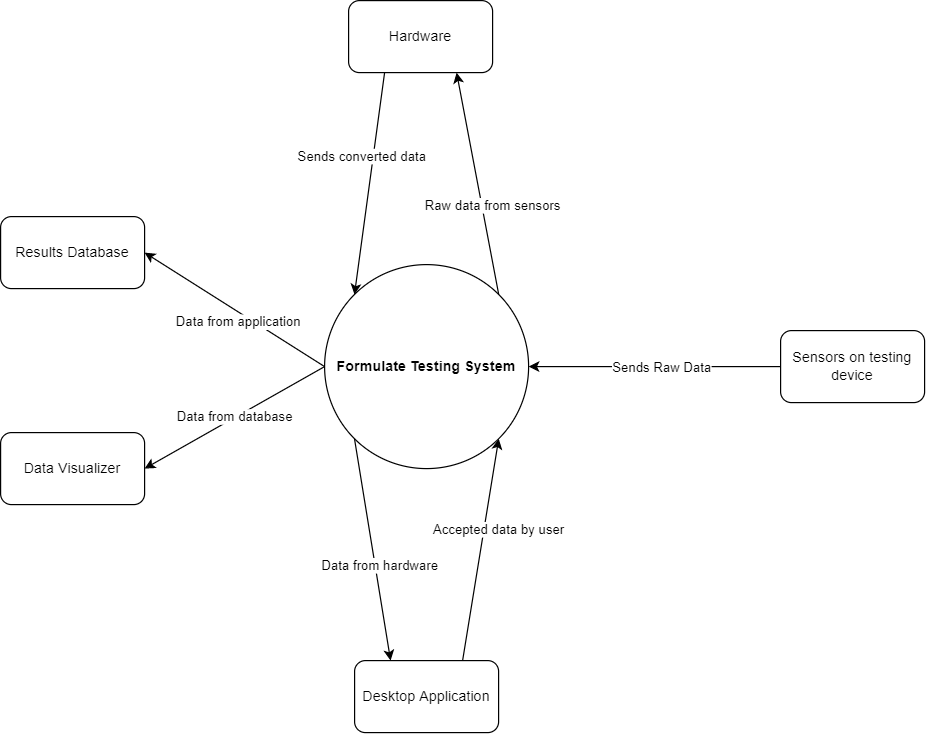
\includegraphics[width=0.9\textwidth]{sys_context_diagram}
\caption{System Context Diagram}
\label{Fig_SystemContext} 
\end{center}
\end{figure}

\subsection{State Transition Diagram}
\begin{figure}[h!]
\begin{center}
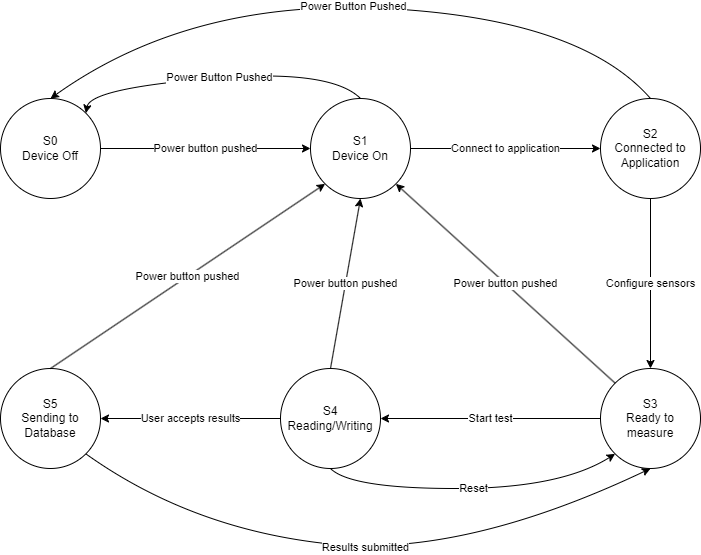
\includegraphics[width=0.8\textwidth]{state_machine_diagram}
\caption{State Machine Diagram}
\label{Fig_StateMachineDiagram} 
\end{center}
\end{figure}

\begin{tabular}{| p{0.23\textwidth} | p{0.66\textwidth}|}
  \hline
  \rowcolor[gray]{0.9}
  State & Description \\
  \hline
  Device Off & The testing device is not powered on\\
  \hline
  Device On &  The testing device is powered on\\
  \hline
  Connected to Application & The testing device has connected to the application \\
  \hline
  Waiting & Waiting for sensor to be inserted so that measurements can begin \\
  \hline
  Reading/Writing & Testing device is reading raw data from sensors, converting them, and sending them to the desktop application \\
  \hline
  Sending to Database & User has accepted the results and they are now sent to the database \\
  \hline
\end{tabular}
\\\\ \indent Table 1.0: State descriptions\\ \\ \\

\subsection{Monitored and Controlled Variables}
  \begin{tabular}{| p{0.23\textwidth} | p{0.10\textwidth}| p{0.10\textwidth}| p{0.46\textwidth}|}
    \hline
    \rowcolor[gray]{0.9}
    Monitored Variable & Type & Units & Description\\
    \hline
    m\_vibration & Analog& V& A signal monitoring the vibration resistance of the motor \\
    \hline
    m\_humidity & Analog & V & A signal monitoring the humidity of the motor’s environment \\
    \hline
    m\_temperature & Analog & V & A signal monitoring the temperature of the motor’s environment \\
    \hline
    m\_shock & Analog & V & A signal monitoring the shock resistance of the motor \\
    \hline
    m\_conv\_vibration & Digital & g  & Converted vibration values that are in useful units \\
    \hline
    m\_conv\_humidity & Digital & \% & Converted humidity values that are in useful units \\
    \hline
    m\_conv\_temperature & Digital & \textdegree C & Converted temperature values that are in useful units \\
    \hline
    m\_conv\_shock & Digital & g & Converted shock values that are in useful units \\
    \hline
    m\_data\_accepted & Digital & T/F & Determines if user has accepted the results and wants to send it to the database \\
    \hline
  \end{tabular}
%\\Table 1.0: Monitored Variables
\\ \\ \\
\begin{tabular}{| p{0.23\textwidth} | p{0.10\textwidth}| p{0.10\textwidth}| p{0.46\textwidth}|}
    \hline
    \rowcolor[gray]{0.9}
    Controlled Variable & Type & Units & Description\\
    \hline
    c\_green\_light& Digital& 1/0& Green LED light on testing device that indicates passed measurements \\
    \hline
    c\_red\_light& Digital & 1/0 & Red LED light on testing device that indicates failed measurements \\
    \hline
    c\_sent\_to\_database & Digital & T/F & Determines if results displayed on the application are sent to the database \\
    \hline
  \end{tabular}
  %\\Table 2.0: Controlled Variables
  \\ \\ \\
  \begin{tabular}{| p{0.23\textwidth} | p{0.10\textwidth}| p{0.10\textwidth}| p{0.46\textwidth}|}
    \hline
    \rowcolor[gray]{0.9}
    Constant & Units & Value & Description\\
    \hline
    k\_temperature\_range& \textdegree C& 5-40& Acceptable ambient temperature values for a Formula Electric motor \\
    \hline
    k\_humidity\_range& \% & 5-85 & Acceptable relative humidity values for a Formula electric motor \\
    \hline
    k\_max\_shock & g & 100 & Maximum shock resistance for a Formula Electric motor \\
    \hline
    k\_max\_vibration & g & 20 & Maximum vibration resistance for a Formula Electric motor \\
    \hline
  \end{tabular}
%  \\Table 3.0: Controlled Variables
\\
\subsection{Functional Decomposition Diagram}
\begin{figure}[h!]
  \begin{center}
  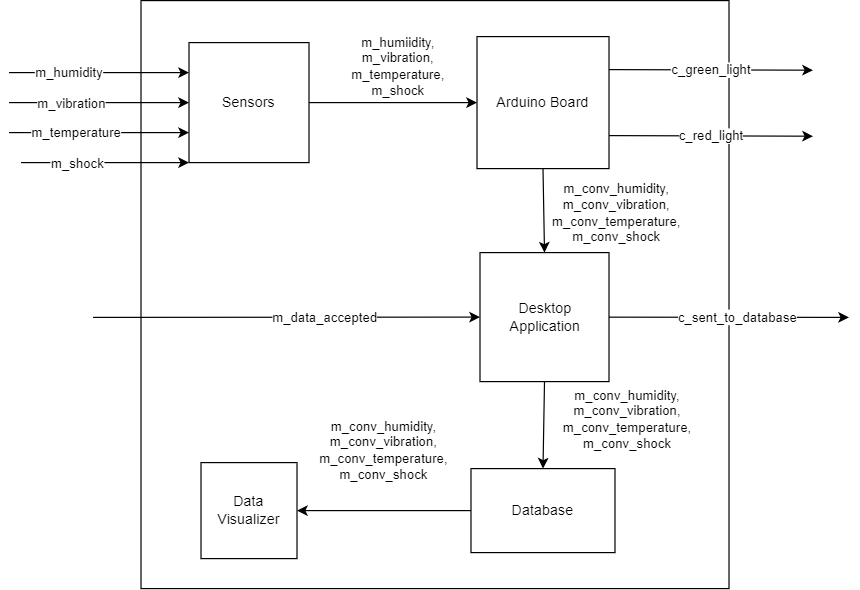
\includegraphics[width=0.9\textwidth]{functional_decomposition}
  \caption{Functional Decomposition Diagram}
  \label{Fig_FunctionalDecomposition} 
  \end{center}
  \end{figure}

\section{Requirements}

\subsection{Functional Requirements}
Formulate consists of 3 main components, each with its own functional requirements. The device addresses the sensors and physical device which interacts directly with the user. The desktop application is the means for the user to select modes and submit data, and the data visualizer (website) is for the user to view old test case data to check if KPI's are met.

\subsubsection{Priority 1} 

\begin{itemize}
  
  \item[FR \refstepcounter{reqnum}\thereqnum:] The device should be able to measure vibration, temperature, humidity, and shock
  
  \item[FR \refstepcounter{reqnum}\thereqnum:] The device should connect to a PC wired to transmit data
  
  \item[FR \refstepcounter{reqnum}\thereqnum:] The device should have a start button which activates the telemetry to start reading values between the PC and device 
  
  \item[FR \refstepcounter{reqnum}\thereqnum:] The device should have a stop button which stops the telemetry stops reading values between the PC and device
  
  \item[FR \refstepcounter{reqnum}\thereqnum:] The device should take the raw data from the sensors and convert it to usable values (g, $^\circ$C, \%)
  
  \item[FR \refstepcounter{reqnum}\thereqnum:] The application should allow users to preview the usable values coming from the device (Temperature, Humidity, Shock, Vibration) after a test

  \item[FR \refstepcounter{reqnum}\thereqnum:] The application should allow the user to send the test results to the database
  
  \item[FR \refstepcounter{reqnum}\thereqnum:] The website should be able to read the test results from the database
  
  \end{itemize}


\subsubsection{Priority 2}
\begin{itemize}

  \item[FR \refstepcounter{reqnum}\thereqnum:] The device's mount to the Formula SAE car should be able to withstand 5g's of force
  
  \item[FR \refstepcounter{reqnum}\thereqnum:] Mounting the device should not take more then 5 minutes

  \item[FR \refstepcounter{reqnum}\thereqnum:] The device should contain a rechargeable battery
  \begin{description} \item[Rationale:] The device needs its own independent power source which will allow for it to be placed in areas without a power socket \end{description}

  \item[FR \refstepcounter{reqnum}\thereqnum:] The device should connect to a PC wirelessly to transmit data

  \item[FR \refstepcounter{reqnum}\thereqnum:] The device should have a screen to display the current status to the user
  
  \item[FR \refstepcounter{reqnum}\thereqnum:] The modular sensors should have a snap on mounting mechanism to connect to the base
  \begin{description} \item[Rationale] Modular sensors need to have a rigid connection with the board with minimal movement to get the most accurate values from the sensor  \end{description}

  \item[FR \refstepcounter{reqnum}\thereqnum:] The application should show live raw data coming from the different sensors (Accelerometer, Thermocouple, Humidity Sensor) during a test
  
  \item[FR \refstepcounter{reqnum}\thereqnum:] The application should allow the user to configure the device's settings
  \begin{description} \item[Rationale:] The device will need to have the wifi setting configured which will be done in the application \end{description}
  
  \end{itemize}

\subsubsection{Priority 3}
\begin{itemize}
  \item[FR \refstepcounter{reqnum}\thereqnum:] The device should have 4 connection ports to add module sensors to it
  \begin{description} \item[Rationale] Each connection port will make the device more modular and allow for users to add more sensors in the future for other tests  \end{description}

  \item[FR \refstepcounter{reqnum}\thereqnum:] The application should allow the user to trim the data before sending it to the database

  \item[FR \refstepcounter{reqnum}\thereqnum:] The website should only allow users who have access to view the data
  
  \item[FR \refstepcounter{reqnum}\thereqnum:] The website should have the option to filter out the data by test conducted
  
  \item[FR \refstepcounter{reqnum}\thereqnum:] The website should show whether the tests passed according to threshold values
  
  \item[FR \refstepcounter{reqnum}\thereqnum:] Any data pushed to the database should not be editable by the user
  
  \item[FR \refstepcounter{reqnum}\thereqnum:] The device should alert the user if any tests exceed the operating condition of the car
  \begin{description} \item[Rationale] If at any point during the test it exceed operating conditions, the devices should make it obvious to the user  \end{description}
  
  \end{itemize}

\newpage
\subsection{Nonfunctional Requirements}

\noindent\begin{itemize}

\subsubsection{Usability} 

    \item[NFR\refstepcounter{nfrnum}\thenfrnum:]
    \textbf{Ease of Learning}\\
    The user will be able to learn the device's operation quickly to integrate into their testing workflow efficiently

    \item[NFR\refstepcounter{nfrnum}\thenfrnum:]
    \textbf{Ease of Use}\\
    The system will be fast at processing data such that additional overhead through the use of the device is less than if all components of the testing workflow were completed individually

\subsubsection{Performance} 

    \item[NFR\refstepcounter{nfrnum}\thenfrnum:]
    \textbf{Speed}\\
    The system bandwidth will be high enough to support testing equipment with high data collection frequencies

    \item[NFR\refstepcounter{nfrnum}\thenfrnum:]
    \textbf{Reliability and Availability}\\
    The system will be fail-safe to withstand single point of failures in components with high probability of operational failure

\subsubsection{Operational}

    \item[NFR\refstepcounter{nfrnum}\thenfrnum:]
      \textbf{Expected Technological Environment}\\
    The device will be able to facilitate a variety of tests using a range of equipment, as long as the equipment is compatible with the data measuring hardware

    \item[NFR\refstepcounter{nfrnum}\thenfrnum:]
    \textbf{Expected Physical Environment}\\
    The system will be operational under a wide range of temperatures and operational vibrations

\subsubsection{Maintainability and Portability}

    \item[NFR\refstepcounter{nfrnum}\thenfrnum:]
      \textbf{Maintainability}\\
    The system will be modular and have low cohesion such that users can adapt elements of the device's hardware and software infrastructure to current needs without breaking other elements

    \item[NFR\refstepcounter{nfrnum}\thenfrnum:]
    \textbf{Portability}\\
    The user's ability to conduct tests will not be affected by the physical constraints from the device
  
\subsubsection{Security}

    \item[NFR\refstepcounter{nfrnum}\thenfrnum:]
    \textbf{Software Integrity}\\
    The system will be secure against malicious spam aimed at reducing validity of aggregate test data stored in the database

\end{itemize}


\subsection{Likely Changes}    

\noindent \begin{itemize}
%Starting and stopping the device to get data using hardware , When the device is connected to the computer we can remote start and stop it using software 
\item[LC\refstepcounter{lcnum}\thelcnum:] Method to start and stop the test on the device
\begin{description} \item[Rationale:] The user should have the ability to perform a hardware start/stop or a remote start/stop from their PC \end{description}
\begin{description} \item[Affected Requirements:] FR3, FR4 \end{description}

\item[LC\refstepcounter{lcnum}\thelcnum:] The initial data we are collecting (Vibration, Shock, Temperature, Humidity)
\begin{description} \item[Rationale:] Since the device is set to be modular, we may change the initial measured values we are testing with other ones \end{description}
\begin{description} \item[Affected Requirements:] FR1 \end{description}

\item[LC\refstepcounter{lcnum}\thelcnum:] The number of modular ports on the device
\begin{description} \item[Rationale:] Depending on the number of input ports available on the board used, the number of input signals available may vary \end{description}
\begin{description} \item[Affected Requirements:] FR15 \end{description}

\end{itemize}

\subsection{Unlikely Changes}    

\noindent \begin{itemize}

\item[ULC\refstepcounter{ulcnum}\theulcnum:] The sensors will remain modular to adapt to different tests that need to be conducted
\begin{description} \item[Rationale:] The product should be expandable in the future to be able to test different values \end{description}
\begin{description} \item[Referenced Requirements:] FR12, NFR5 \end{description}

\item[ULC\refstepcounter{ulcnum}\theulcnum:] The communication methods between the data measurement hardware and the PC will be wired or wireless
\begin{description} \item[Referenced Requirements:] FR10 \end{description}

\end{itemize}

\subsection{Traceability Table}

  \begin{tabular}{| p{0.3\textwidth} | p{0.3\textwidth}| p{0.33\textwidth}|}
    \hline
    \rowcolor[gray]{0.9}
    Section & Functional Requirements & Non-Functional Requirements\\
    \hline
    Hardware & FR 1, FR 2, FR 3, FR 4, FR 8, FR 9, FR 10, FR 11, FR 12, FR 15, FR 21 & NFR 1, NFR 2, NFR 4, NFR  5, NFR 6, NFR 7, NFR 8 \\
    \hline
    Desktop Application & FR 5, FR 6, FR 13, FR 14, FR 16 & NFR 1, NFR 2, NFR 3, NFR 7, NFR 9\\
    \hline
    Database & FR 20 & NFR 7, NFR 9\\
    \hline
    Data Visualizer & FR 7, FR 17, FR 18 & NFR 1, NFR 2, NFR 7\\
    \hline
  \end{tabular}
%\\Table 1.0: Monitored Variables
\\

\section{Phase in Plan}

The phase in plan is categorized into multiple sections, where each section represented a significant phase in the progress of project execution. A section is given a number in the hundreds (X00) to denote a significant phase in the project. Each section is subdivided further into segments given by numbers specified in the tens (XX0) to denote smaller steps within each phase. The expected order of segment completion follows the order of increasing number count; the lowest number segment should be completed first and the highest number segment should be completed last.\\

Each segment has an overall goal that can include the coordination of multiple team members. Upon completion of each segment, the team members relevant to the segment will review and buyoff the readyness of the segment. Upon completion of buying off each segment within a section, the overall phase is considered to be bought off and completed with confidence. The relevant stakeholders must aim to buyoff each segment in a phase before the phase deadline.\\

ADD SECTION RELATING PRIORITIES FROM FUNCTIONAL REQUIREMENTS TO X00 BUYOFFS

\noindent
\subsection{Phase 0: Preperation (000 Series)}
Phase 0 Deadline: October 28, 2022\\

\begin{table}[H]
  \centering
  \begin{tabular}{|p{2cm}|p{10cm}|p{2cm}|}
  \hline
  \multicolumn{1}{|c|}{\textbf{000 Buyoffs}} & \multicolumn{1}{c|}{\textbf{Explanation}} & \multicolumn{1}{|c|}{\textbf{Stakeholder(s)}}
  \\ \hline
  010
  & Purchase sensor equipment, data measurement hardware, 3D print material.
  & Stephen
  \newline                                
  \\ \hline

  020                              
  & Obtain licenses for 3D CAD software use and database access
  & Stephen
  \newline                                
  \\ \hline

  030                          
  & Document material costs and licensing constraints
  & Stephen
  \newline                                
  \\ \hline

  040                                
  & Distribute materials and licensing to relevant project area Stakeholder
  & Stephen 
  \newline                            
  \\ \hline

  050                                
  & Completion of device chassis mechanical design and modelling
  & Stephen 
  \newline                            
  \\ \hline

  060                                
  & Completion of electrical connection hardware circuit design and schematic
  & Stephen 
  \newline                            
  \\ \hline

  090                                
  & Device chassis manufactured
  & Stephen 
  \newline                            
  \\ \hline

  \end{tabular}
\end{table}
\newpage

\noindent
\subsection{Phase 1: Proof of Concept (100 Series)}
Phase 1 Deadline: November 11, 2022\\
\begin{table}[H]
  \centering
  \begin{tabular}{|p{2cm}|p{10cm}|p{2cm}|}
  \hline
  \multicolumn{1}{|c|}{\textbf{100 Buyoffs}} & \multicolumn{1}{c|}{\textbf{Explanation}} & \multicolumn{1}{|c|}{\textbf{Stakeholder(s)}}
  \\ \hline
  110
  & Desktop application program developed with basic user interface
  & Stephen
  \newline                                
  
  \\ \hline
  120                              
  & Desktop application program can recieve data from data measurement device using a wired connection
  & Stephen
  \newline                                

  \\ \hline
  130                          
  & Desktop application program can interface with database to send data
  & Stephen
  \newline                                

  \\ \hline
  140                                
  & Desktop application program can edit data from data measurement device before sending it to the database
  & Stephen 
  \newline                            

    \\ \hline
  150                                
  & Visualization application can pull data and generate KPI metrics from the database
  & Stephen 
  \newline 

  \\ \hline
  160                                
  & Integration between data measurement device and desktop application
  & Stephen 
  \newline 

  \\ \hline
  170                                
  & Integration between desktop application and visualization application
  & Stephen 
  \newline 

  \\ \hline
  190                                
  & Integration between data measurement device, desktop application, and data measurement device
  & Stephen 
  \newline 
  \\ \hline


  \end{tabular}
\end{table}

\newpage
\noindent
\subsection{Phase 2: Revision 0 Presentation (200 series)}
Phase 2 Deadline: February 3, 2023\\

\begin{table}[H]
  \centering
  \begin{tabular}{|p{2cm}|p{10cm}|p{2cm}|}
  \hline
  \multicolumn{1}{|c|}{\textbf{200 Buyoffs}} & \multicolumn{1}{c|}{\textbf{Explanation}} & \multicolumn{1}{|c|}{\textbf{Stakeholder(s)}}
  \\ \hline
  210
  & Mechanical design and modelling completion of physical user interface components on device chassis and connection modules
  & Stephen
  \newline                                
  \\ \hline

  220                              
  & Completion of wireless communication between data measurement device and desktop application 
  & Stephen
  \newline                                
  \\ \hline

  230                          
  & Completion of database security against tests that break utility of database
  & Stephen
  \newline                                
  \\ \hline

  290                                
  & Completion of extended KPI features for visualization application
  & Stephen 
  \newline                            
  \\ \hline

  \end{tabular}
\end{table}
\newpage

\noindent
Phase 3: Final Demonstrations (300 series)\\
Phase 3 Deadline: March 17, 2023\\


\section{Appendix}

\subsection{Knowledge Requirement}
\begin{enumerate}
  \item \textbf{Sensors/Embedded Systems:} To successfully complete this project our group needs to collectively understand how sensors and microcontrollers work. The main premise of our project is to automate testing of key components in a Formula Electric vehicle, this can only be done using a variety of sensors to monitor those components. To create almost any hardware device sensors are required as it is equivalent to being the eyes of the device, it allows for hardware to understand and map it's environment. These measurements that the sensor collects can be used by a microcontroller to make decisions on what to do according to the requirements. In our project specifically our hardware device needs to collect measurements from its environment and react accordingly with it, (i.e transmit it to a PC, alert the user if thresholds are exceeded, etc.)
  
  \item \textbf{Project Management:} STEPHEN
  
  \item \textbf{Databases:} An essential function of Formulate is to collect test results and store them in a database. Therefore, a complete understanding of creating, accessing, securing, and editing databases is required to achieve that functionality. We are aiming to use a relational database, so all research on these topics will specific to relational databases.
  
  \item \textbf{Presentations:} For our presentation we will all play a part in presenting and demonstrating how our new device. In our presention we will require the knowledge of how the device works and the usefulness of our device. Our knowledge will be learnt throughout the making of our capstone project as we get more familiar with its software and hardware components. Our presentation will be a demonstration of our knowledge as we will show how we made it and how it is uniquely designed by us. In order for our presentation to be a success we will have practice and create a unique way to entertain our audience. This will require creativity from us so we can stand out from the rest of the presentations, which we will discuss more and more during our weekly meetings. 
  
\end{enumerate}


\subsection{Knowledge Acquirement }

\begin{enumerate}
  \item \textbf{Sensors/Embedded Systems:} There are many resources to help in mastering the skill, McMaster provides access to a platform called LinkedIn Learning, it provides useful relevant courses to programming an Arduino and how to use sensors. Other online resources such as YouTube also provides similar knowledge in these topics. The best way to learn something in my opinion is by experimenting with the technology, this is called the discovery phase. Getting familiar with the technology by messing around with it drastically improves how comfortable you are with it and how to use it. Ahmed will pursue this because he has some relevant coop experience in sensors and embedded systems and he would like to get more hands on experience working on these technologies. These skills are relevant to the type of work he wants to do in the future.
  
  \item \textbf{Project Management:} STEPHEN
  
  \item \textbf{Databases:} Muhanad is currently taking a databases course (3DB3) at McMaster which is an introduction to all the fundamentals of relational databases. This includes the design and creation of legal databases based on relational constraints and the manipulation of data using SQL (Structured Query Language). This course will be very useful in terms of creating a fundamentally sound database. However, online resources will be used to determine where to host a database and how to make it secure in a way where only the application has write access to it. Muhanad is pursuing databases because he interacted with them briefly during his coop and found SQL to be very interesting. Therefore, he wishes to take a more in-depth look at databases and querying languages to gain a full understanding of them.
  
  \item \textbf{Presentations:} In order to master the art of presentations you can take advice from difference audiences on what they like when someone is presenting something to them. The main focus is to keep the audience engaged and make sure they understand the presentation, feedback from different audiences will always help since you will see what audiences like to when watching a presentation and what keeps them engaged. Another way to master the skill of presentation is to watch notable presenters and speakers and see how they keep their audiences engage and make it easy for them to understand. For our method we will look at other presentations and critique what they did well and what they could improve and compare it to ours to see how we could improve our presentation and what to avoid when presenting our product.
  
\end{enumerate}

\newpage

\bibliographystyle {plainnat}
\bibliography {../../refs/References}

\newpage

\noindent \plt{The following is not part of the template, just some things to consider
  when filing in the template.}

\noindent \plt{Grammar, flow and \LaTeX advice:
\begin{itemize}
\item For Mac users \texttt{*.DS\_Store} should be in \texttt{.gitignore}
\item \LaTeX{} and formatting rules
\begin{itemize}
\item Variables are italic, everything else not, includes subscripts (link to
  document)
\begin{itemize}
\item \href{https://physics.nist.gov/cuu/pdf/typefaces.pdf}{Conventions}
\item Watch out for implied multiplication
\end{itemize}
\item Use BibTeX
\item Use cross-referencing
\end{itemize}
\item Grammar and writing rules
\begin{itemize}
\item Acronyms expanded on first usage (not just in table of acronyms)
\item ``In order to'' should be ``to''
\end{itemize}
\end{itemize}}

\noindent \plt{Advice on using the template:
\begin{itemize}
\item Difference between physical and software constraints
\item Properties of a correct solution means \emph{additional} properties, not
  a restating of the requirements (may be ``not applicable'' for your problem).
  If you have a table of output constraints, then these are properties of a
  correct solution.
\item Assumptions have to be invoked somewhere
\item ``Referenced by'' implies that there is an explicit reference
\item Think of traceability matrix, list of assumption invocations and list of
  reference by fields as automatically generatable
\item If you say the format of the output (plot, table etc), then your
  requirement could be more abstract
\end{itemize}
}

\end{document}